\chapter{Estado del arte}

A continuación, se hace un repaso de la tecnología existente en la actualidad relacionada con los campos tocados por el presente proyecto. El objetivo es proporcionar al lector un punto de partida del trabajo y comentar las soluciones utilizadas por otros autores. 

\section{Water level control using Raspberry Pi + XBee + XBMQ + MQTT + Node-Red \cite{zhivazhiva:RaspberryPi}}

Se trata de un proyecto que trabaja de manera bastante similar al trabajo objetivo del presente documento, teniendo ciertas tecnologías en común.

El objetivo es el control de una pequeña bomba de agua que llena un depósito lentamente, con una distancia considerable entre ambos elementos y el ordenador central. La motivación para automatizar el proceso de llenado del depósito era evitar ciertos incidentes provocados por el olvido de la persona que controlaba la bomba, debido a los extensos tiempos que se tomaba el sistema para llenar el depósito. El autor comenta que la señal se perdía frecuentemente al usar unos módulos Wi-Fi baratos y terminó decidiéndose por la tecnología XBee de Digi, descartando cualquier tecnología que no fuera inalámbrica por los motivos de distancia comentados previamente.

\begin{figure}[tb]
\centering
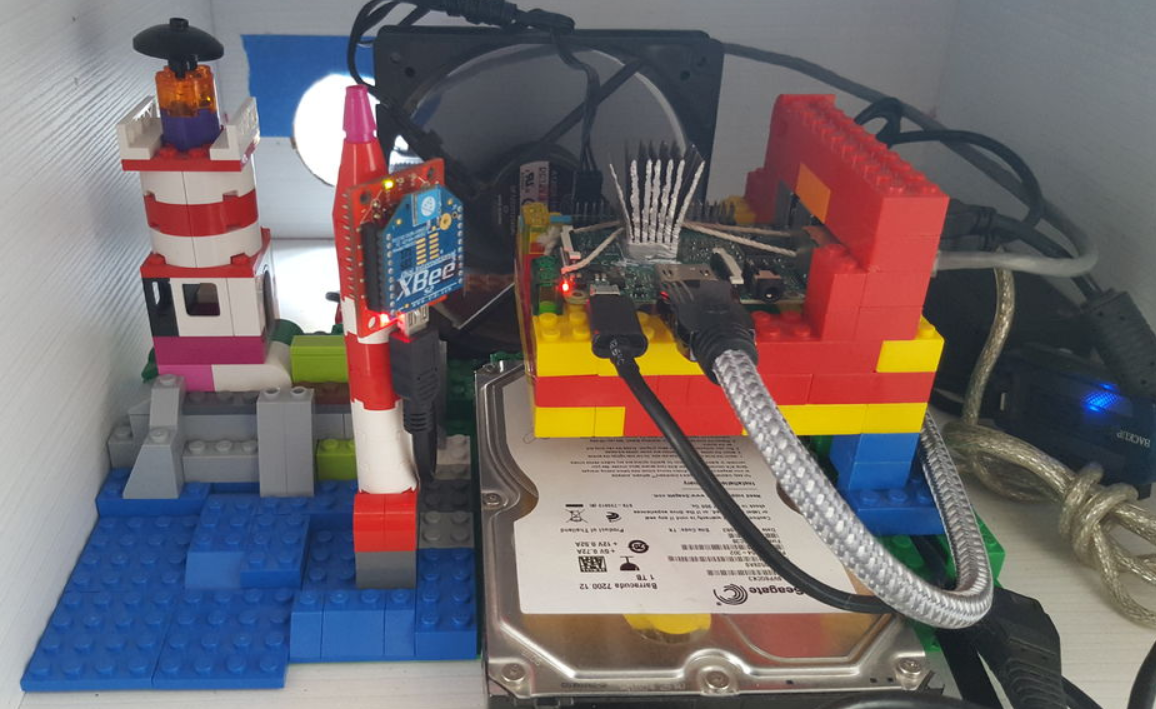
\includegraphics[width=0.55\textwidth]{figuras/EArte1.png}
\caption{Montaje del proyecto 3.1}
\label{fig:EArte1}
\end{figure}

Una Raspberry Pi3 ejerce de ordenador central del sistema y es el componente encargado de coordinar la interacción con el usuario que manda la orden y la interacción con el depósito y la bomba de agua vía XBee (montaje en la figura \ref{fig:EArte1}).

\begin{itemize}
\item Por un lado, tiene instalado Mosquitto (MQTT); un programa que usa la red para crear una especie de "tablón de anuncios" virtual. Los dispositivos conectados a esa red pueden suscribirse a un \textit{topic} y recibir lo que otros dispositivos publican en él.
La idea es que, haciendo uso de diferentes aplicaciones (como puede ser el caso de \textit{IoT MQTT Dashboard} en Android), se puedan publicar ciertos mensajes en algún \textit{topic} al que esté suscrita la Raspberry Pi desde otros dispositivos de manera remota. La Raspberry recibe esta información y actúa en consecuencia.
\item XBMQ actúa de puente dentro de la Raspberry Pi entre MQTT y el módulo XBee conectado a la misma, que es el que se comunica con el actuador y el sensor.
\item La Raspberry Pi envía los comandos al actuador y recibe la información del sensor a través del módulo XBee. En el lado del depósito, se sitúa el otro XBee con una salida controlando un pequeño relé que acciona y desactiva la bomba y una entrada que envía al XBee de la Raspberry el estado del sensor. Huelga mencionar que ambos XBee se han debido configurar adecuadamente.
\item Para detener la bomba si el sensor detecta que el depósito está lleno, se precisa de cierta lógica que se programa en la Raspberry usando otra tecnología que se verá mas en detalle: Node-Red. El uso de este programa permite automatizar otras acciones paralelas como, por ejemplo, publicar un tweet cada vez que la bomba cambie de estado.
\end{itemize}

\section{Servidor Raspberry Pi-XBee en Python \cite{JONIUZ:IoT}}

El proyecto detalla la conexión de un Arduino Uno y una Raspberry Pi a través de XBee. Viene siendo algo muy similar a una de las etapas del trabajo detallado en este documento.

En el lado del Arduino Uno, emplea una XBee Shield 2.0 de Sheeed Studio (figura \ref{fig:EArte2}) para implemental el módulo de radio frecuencia.

\begin{figure}[tb]
\centering
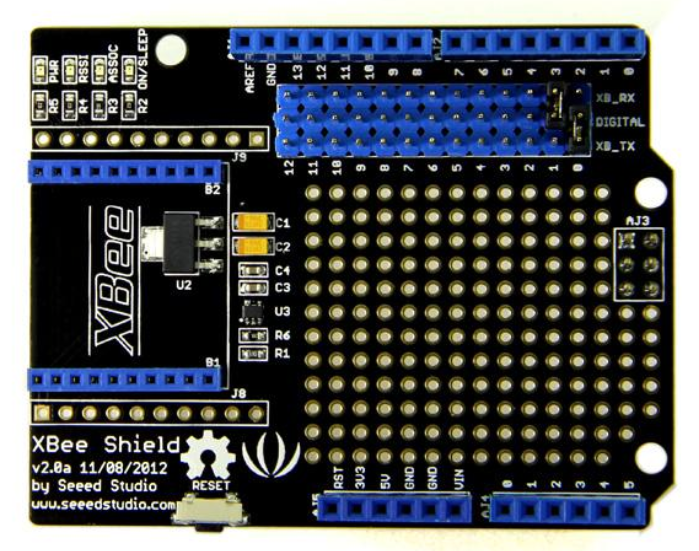
\includegraphics[width=0.55\textwidth]{figuras/EArte2.png}
\caption{XBee Shield v2.0 - Seeed Studio}
\label{fig:EArte2}
\end{figure}

Si se habla del lado de la Raspberry Pi, la interacción con el módulo XBee se realiza a través de una placa XBee Explorer.

Como uno puede comprobar, existe una gran variedad de placas y shields que adaptan y facilitan la interacción de los módulos XBee con las plataformas de ordenadores y microcontroladores más populares.

En este caso, los módulos XBee están configurados como AT. Más adelante en el documento se detalla esta cualidad.

\section{Smart Porch Light Project \cite{SPLP:Mouser}}

En el contexto del Internet de las Cosas (IoT), el autor desarrolla un proyecto de red inalámbrica de sensores y actuadores sincronizados a una nube en la red.

El caso particular consta de una luz de exterior que es automáticamente controlada teniendo en cuenta los datos obtenidos de múltiples sensores que captan el estado del entorno. Estos sensores miden la luz ambiente, temperatura, humedad y luz ultravioleta. El control de la lámpara de exterior se lleva a cabo con un relé capaz de separar la etapa de potencia de la etapa de señal. Con el proyecto operativo, se usan servicios en la nube para almacenar y leer la información del estado del sistema; obteniendo como resultado una lámpara inteligente que permite mostrar a los usuarios el estado de los sensores desde cualquier dispositivo con acceso a internet.

Los componentes hardware, al ser todos del mismo fabricante (Seeed Studio), permiten su apilamento en un único stack compacto (figura \ref{fig:EArte4}) de microcontrolador, shields módulo XBee. El microcontrolador es un Arduino Mega, los shields son de sensores y de XBee y,coronando el stack, se encuentra el módulo XBee LTE.

\begin{figure}[t]
\centering
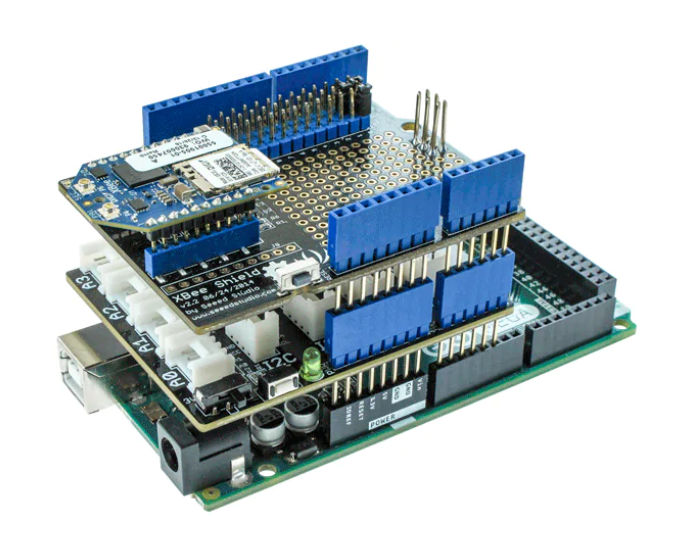
\includegraphics[width=0.55\textwidth]{figuras/EArte4.png}
\caption{Stack Hardware del proyecto 3.4}
\label{fig:EArte4}
\end{figure}

A diferencia de proyectos mencionados anteriormente, en este se usa una API REST en lugar de MQTT para transferir la información al servicio de nube correspondiente y los módulos XBee son del modelo LTE, por lo que pueden acceder a la red directamente sin la necesidad de poseer enlace alguno a un ordenador con conexión, bien vía USB o a través de otro módulo XBee. Por otro lado, la interfaz donde mostrar el estado de los sensores no se basa en Node-RED, sino en Ubidots.

\section{Home Automation System \cite{Molnar:Digi}}

Estamos ante otro proyecto del campo IoT que hace uso de módulos XBee. En este caso, los actuadores y sensores de una casa en la que se ha implementado este sistema domótico están conectados a red inalámbrica de módulos XBee mediante cableados como el que se muestra en la figura \ref{fig:EArte5}.

\begin{figure}[tb]
\centering
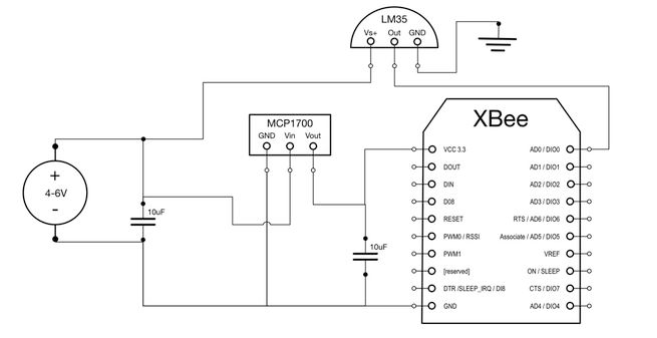
\includegraphics[width=0.55\textwidth]{figuras/EArte5.png}
\caption{Esquema de conexión del sensor de temperatura}
\label{fig:EArte5}
\end{figure}

La información se transmite a un portal central que tiene como base una placa Netduino o una Raspberry Pi con Windows IoT como sistema operativo. El portal envía y recibe mensajes de cada uno de los módulos XBee conectados y traduce la información de tal manera que el controlador lo pueda interpretar.

Usa MQTT para la comunicación controlador-portal pero recurre a una nueva herramienta, openHAB, para proporcionar una interfaz gráfica donde monitorizar y controlar los sensores y actuadores de la casa.

\section{Controlador central para un sistema domótico utilizando el protocolo inalámbrico ZigBee \cite{ULL:2016}}

Con este proyecto se habla del desarrollo de otro sistema domótico; esta vez basado en la placa de desarrollo Pandaboard (figura \ref{fig:EArte6}). A principios de la presente década, Pandaboard nació para competir en el mercado de los ordenadores pequeños de bajo coste, pero Raspberry terminó por dominar a la competencia. Hoy en día se trata de una placa obsoleta y poco usada por la comunidad.

\begin{figure}[tb]
\centering
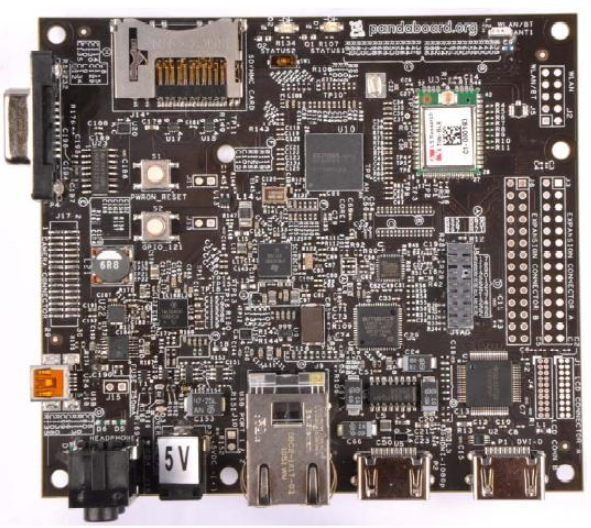
\includegraphics[width=0.55\textwidth]{figuras/EArte6.png}
\caption{PandaBoard ES}
\label{fig:EArte6}
\end{figure}

En este proyecto se recurre también al uso de dispositivos XBee para la transmisión de información y a MQTT. Incorpora Domoticz, un programa de supervisión y configuración domótica de código abierto.

Como particularidad de la que se hablará de manera mas detallada más adelante, en este caso los módulos XBee funcionan en configuración API, en contraposición al modo AT mencionado previamente en otro proyecto.

\section{Node-RED based custom full-room wake-up light \cite{Bulten:2019}}

Proyecto que desarrolla una aplicación Node-RED con el fin de configurar un patrón despertador configurable. El desarrollo del proyecto referenciado \cite{Bulten:2019} se centra en la definición de los flujos de Node-RED puesto que el sistema domótico se ha desarrollado previamente \cite{Bulten:2018}.

El flujo de Node-RED (figura \ref{fig:EArte7}) trabaja detectando la igualdad entre la hora programada y la actual. A continuación, comprueba si es fin de seamana y si está activada la alarma durante los fines de semana en la configuración. Por último y habiendo superado las etapas anteriores, se define una secuencia de iluminación de las bombillas correspondiente a la señal de despertador.

\begin{figure}[tb]
\centering
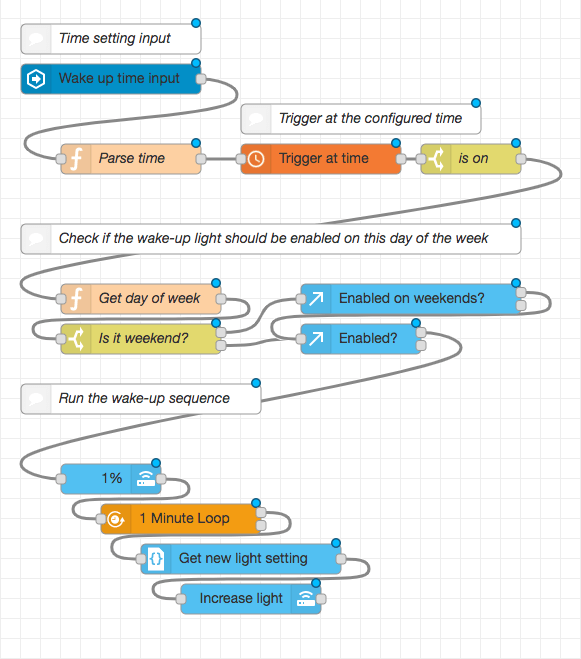
\includegraphics[width=0.75\textwidth]{figuras/EArte7.png}
\caption{Flujo de Node-RED}
\label{fig:EArte7}
\end{figure}

El proyecto domótico completo se basa en una instalación de Node-RED y Home Assistant, que proporciona la interfaz de usuario, sobre una Raspberry Pi. Las bombillas son bombillas inteligentes que reciben ordenes vía XBee. La recepción y envío de radiofrecuencia desde la Raspberry Pi se produce a través de un hub comercial que va alternando la conexión con las diferentes bombillas a muy alta velocidad.

\section{ArduSmartHome \cite{UOC:2017}}

El proyecto ArduSmartHome consiste en el desarrollo de un sistema domótico de control que capture datos del entorno a través de varios sensores y monitorizar esa información usando Node-RED.

La principal diferencia que tiene este proyecto con los mencionados previamente es la tecnología usada para la transmisión de la información. Mientras que hasta ahora se habiía usado principalmente radiofrecuencia a través de módulos XBee\footnote{La tecnología utilizada en el proyecto que describe este documento es, precisamente, radiofrecuencia usando módulos XBee}, en este caso se usa una red WiFi local.

\begin{figure}[tb]
\centering
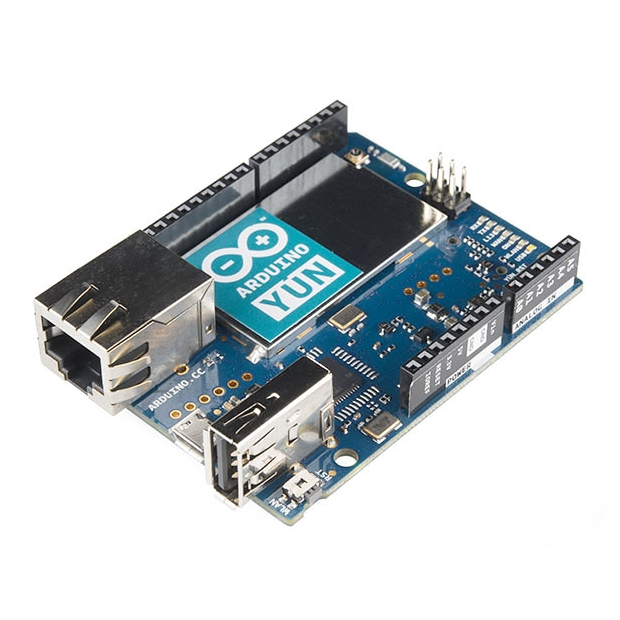
\includegraphics[width=0.55\textwidth]{figuras/EArte8.png}
\caption{Arduino Yun}
\label{fig:EArte8}
\end{figure}

Para conseguir esto, se hace uso de un microcontrolador diseñado para esta tarea, el Arduino Yun (figura \ref{fig:EArte8}). La red domótica posee varios de estos microcontroladores volcando los datos de los sensores que tienen conectados a la red local. Existe un Arduino Yun\footnote{Se puede lograr una equivalencia económica al Arduino Yun usando un Arduino UNO complementado con la shield de extensión Dragino Yun Shield v2.4} que ejerce las funciones de coordinador de las comunicaciones a la vez que es quién se encarga de establecerlas. En este proyecto también se hace uso de MQTT.

\section{University of Minnesota – Solar Vehicle \cite{UM:SV}}

Estudiantes de la Universidad de Minnesota llevan desde 1990 desarrollado prototipos de coches solares para competir en varios certámenes a nivel nacional e internacional, obteniendo grandes resultados. En este contexto, en 2019 se ha presentado el nuevo prototipo denominado EOS II (figura \ref{fig:EArte3}). 

\begin{figure}[b]
\centering
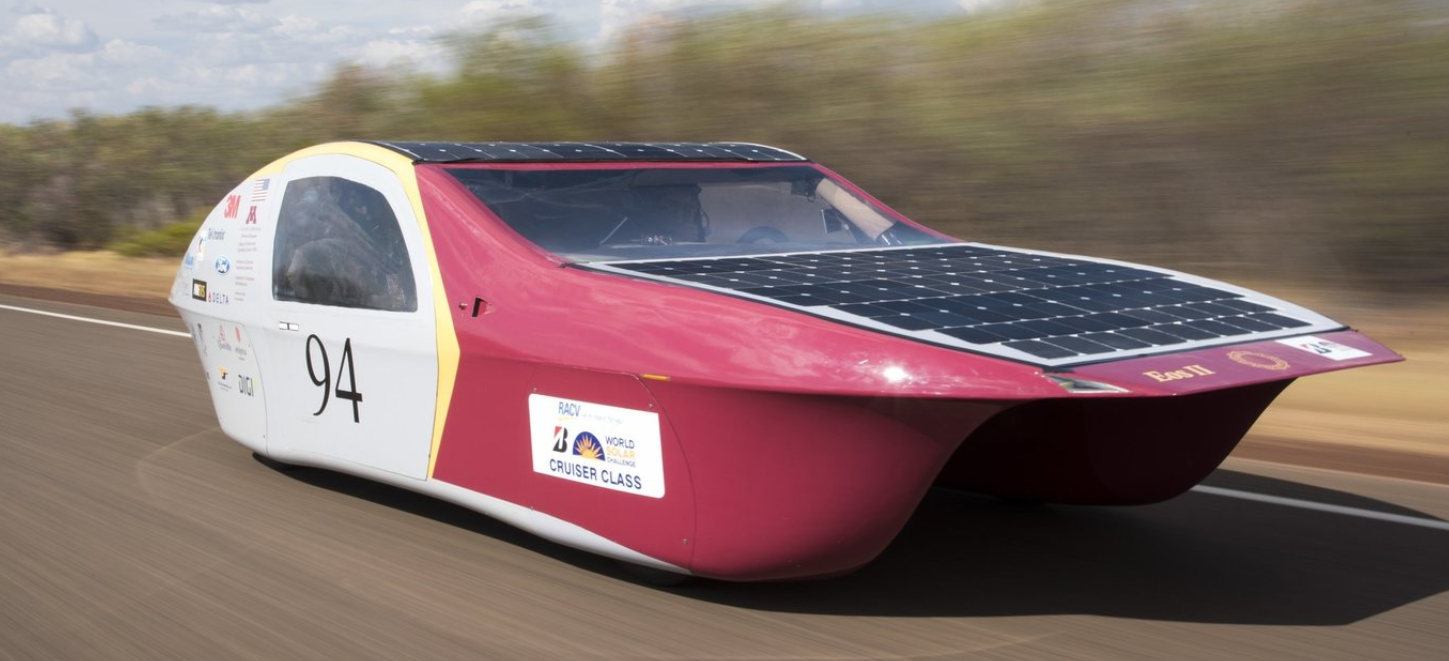
\includegraphics[width=0.55\textwidth]{figuras/EArte3.png}
\caption{EOS II Solar car}
\label{fig:EArte3}
\end{figure}

Con el apoyo de Digi, han implementado una red inalámbrica a la que conectan ordenadores y diferentes sensores. La conexión a esta red se realiza mediante módulos XBee. El objetivo final es la comunicación entre los módulos para la detección de errores y el almacenamiento de los datos adquiridos por esos mismos sensores durante el funcionamiento del prototipo.